\documentclass[11pt]{amsart}

% Encoding and fonts
\usepackage[T1]{fontenc}
\usepackage[utf8]{inputenc}
\usepackage{lmodern}

% Math packages
\usepackage{amsmath}
\usepackage{amssymb}
\usepackage{amsfonts}
\usepackage{amsthm}
\usepackage{mathtools}

% Layout and utilities
\usepackage{geometry}
\usepackage{enumitem}
\usepackage{booktabs}
\usepackage{pgfplots}
\usepackage{caption}

\geometry{margin=1in}

\numberwithin{equation}{section}
\setcounter{tocdepth}{3}
\setcounter{secnumdepth}{3}

\pgfplotsset{compat=1.18}

% ---------------------------------------------------------
% Theorem-like environments
% ---------------------------------------------------------

\theoremstyle{plain}
\newtheorem{theorem}{Theorem}[section]
\newtheorem{proposition}[theorem]{Proposition}
\newtheorem{lemma}[theorem]{Lemma}
\newtheorem{corollary}[theorem]{Corollary}
\newtheorem{conjecture}[theorem]{Conjecture}

\theoremstyle{definition}
\newtheorem{definition}[theorem]{Definition}
\newtheorem{experiment}[theorem]{Experiment}
\newtheorem{heuristic}[theorem]{Heuristic}
\newtheorem{question}[theorem]{Question}

\theoremstyle{remark}
\newtheorem{remark}[theorem]{Remark}
\newtheorem{warning}[theorem]{Warning}

% Hyperref last
\usepackage[hidelinks]{hyperref}

\title{
Residual Structure Does Not Account for the Raw Modular Excess
in Zeta-Zero Gaps
}

\author{Rôtkiv Aynäsac}
\date{June 15, 2026}

\begin{document}

\maketitle

\tableofcontents

\bigskip

\begin{remark}
\label{rem:exploratory_nature}
This notebook is exploratory in nature.
Its purpose is to record and organise numerical experiments on
nearest-neighbour gaps between nontrivial zeros of the Riemann zeta function,
with a particular focus on two aspects:
the residuals of a smooth reference model and
the modular distribution of raw gaps.
Several sections contain formal manipulations, heuristic arguments,
and speculative interpretations.
Whenever a statement is rigorous it will be explicitly identified as such.
All remaining claims should be regarded as tentative, heuristic, or conjectural.
\end{remark}

\section{Objects and notation}
\label{sec:objects_notation}

Let
\begin{equation}
\rho_k = \tfrac12 + i\gamma_k
\label{eq:rho_k_definition}
\end{equation}
denote the $k$-th nontrivial zero of the Riemann zeta function on the
critical line, assuming the Riemann Hypothesis for notational convenience.
We write
\begin{equation}
Y_k = \gamma_k
\label{eq:Yk_definition}
\end{equation}
for the ordinates and
\begin{equation}
G_k = Y_{k+1} - Y_k
\label{eq:Gk_definition}
\end{equation}
for the raw nearest-neighbour gaps.

\begin{remark}
\label{rem:standard_zero_notation}
The notation in \eqref{eq:rho_k_definition}--\eqref{eq:Gk_definition}
is standard and consistent with classical references such as
\cite{Titchmarsh1986,Edwards2001}.
No new assumptions are introduced here.
\end{remark}

We consider a smooth reference model for the ordinates,
denoted
\begin{equation}
\gamma_k^{\mathrm{RVM}},
\label{eq:RVM_definition}
\end{equation}
and define the residuals
\begin{equation}
R_k = \gamma_k - \gamma_k^{\mathrm{RVM}}.
\label{eq:Rk_definition}
\end{equation}
The corresponding residual jumps are
\begin{equation}
\Delta R_k = R_{k+1} - R_k.
\label{eq:dR_definition}
\end{equation}

\begin{remark}
\label{rem:RVM_informal}
The precise construction of the reference model
$\gamma_k^{\mathrm{RVM}}$ in \eqref{eq:RVM_definition}
is not needed for the present notebook.
We treat it as a smooth approximation to the ordinates
whose residuals $R_k$ and jumps $\Delta R_k$ can be computed numerically.
\end{remark}

For the modular analysis of raw gaps we consider the fractional parts
\begin{equation}
x_k = \{ Y_{k+1} - Y_k \} \in [0,1),
\label{eq:xk_definition}
\end{equation}
and study the first circular harmonic of their empirical distribution.

\section{Summary of the residual/gap matrix study}
\label{sec:matrix_study_summary}

This section records the main numerical outputs of the
``matrix study of residuals/gaps''.
The underlying computations are local in $k$ and use
the first $51$ residuals and $50$ residual jumps.

\subsection{Basic statistics}
\label{subsec:basic_statistics}

The study reports the following summary statistics for the residuals
and their jumps:
\begin{align}
\mathbb{E}[R_k] &\approx -1.3201457,
\label{eq:mean_R}\\
\operatorname{std}(R_k) &\approx 0.66974925,
\label{eq:std_R}\\
\operatorname{std}(\Delta R_k) &\approx 0.87518461.
\label{eq:std_dR}
\end{align}

\begin{experiment}
\label{exp:residual_basic_stats}
The quantities in \eqref{eq:mean_R}--\eqref{eq:std_dR}
are computed from the first $51$ residuals $R_k$
and the first $50$ jumps $\Delta R_k$.
Empirically one finds a negative mean residual and
standard deviations of order $1$ for both $R_k$ and $\Delta R_k$.
\end{experiment}

\subsection{Feature correlation matrix}
\label{subsec:feature_correlation}

The matrix study considers five features,
which we denote symbolically by
\begin{equation}
(dG, dRVM, dR, SG, SR),
\label{eq:feature_list}
\end{equation}
and reports the empirical correlation matrix
\begin{equation}
C =
\begin{pmatrix}
1.00 & 0.69 & 0.82 & 0.76 & 0.76 \\
0.69 & 1.00 & 0.15 & 0.08 & 0.07 \\
0.82 & 0.15 & 1.00 & 0.98 & 0.97 \\
0.76 & 0.08 & 0.98 & 1.00 & 1.00 \\
0.76 & 0.07 & 0.97 & 1.00 & 1.00
\end{pmatrix}.
\label{eq:feature_correlation_matrix}
\end{equation}

\begin{experiment}
\label{exp:feature_correlation}
The matrix \eqref{eq:feature_correlation_matrix}
shows that $dR$ is strongly correlated with $SG$ and $SR$
(correlations $0.98$ and $0.97$),
while $dRVM$ has only weak correlation with $dR$
(correlation $0.15$).
This indicates that the residual jumps $\Delta R_k$
are not linearly controlled by the smooth model increments $dRVM$,
but they are tightly linked to the gap-related features $SG$ and $SR$.
\end{experiment}

\subsection{Local PCA of features}
\label{subsec:local_pca_features}

A principal component analysis of the five-dimensional feature vector
\eqref{eq:feature_list} yields that the first two principal components
explain essentially all of the variance:
\begin{align}
\text{PC1 variance share} &\approx 74.82\%,
\label{eq:PC1_feature}\\
\text{PC2 variance share} &\approx 24.50\%,
\label{eq:PC2_feature}\\
\text{PC1+PC2 variance share} &\approx 99.323\%.
\label{eq:PC12_feature}
\end{align}

\begin{remark}
\label{rem:feature_pca_rank}
The near saturation in \eqref{eq:PC12_feature}
suggests that the local feature cloud
is effectively two-dimensional in the PCA sense.
This is a structural observation about the joint distribution of
$(dG,dRVM,dR,SG,SR)$, but it does not by itself imply
any simple temporal dynamics for the residuals.
\end{remark}

\subsection{Hankel singular values of residual jumps}
\label{subsec:hankel_singular_values}

The Hankel matrix built from the residual jumps $\Delta R_k$
is analysed via its singular values.
The study reports that the leading singular value accounts for
\begin{equation}
\sigma_1 \approx 10.193\%,
\label{eq:hankel_sigma1_share}
\end{equation}
and the first five singular values together account for
\begin{equation}
\sigma_1 + \cdots + \sigma_5 \approx 45.730\%.
\label{eq:hankel_sigma1_5_share}
\end{equation}

In logarithmic scale, the singular values are given (for the first few)
by
\begin{equation}
\log_{10}(\sigma_j) \approx
1.15,\ 0.417,\ -0.316,\ -1.05,\ -1.78,\ -2.52,\ \dots
\label{eq:hankel_log_singular_values}
\end{equation}
for $j=1,2,\dots$.

\begin{experiment}
\label{exp:hankel_singular_values}
The Hankel singular spectrum of $\Delta R_k$
does not collapse to rank one:
the leading singular value carries only about $10\%$ of the total weight,
and the first five together less than $50\%$.
This indicates that the residual jumps do not exhibit
a dominant low-rank temporal structure.
\end{experiment}

We now include a PGFPlots figure for the logarithmic singular values
reported in \eqref{eq:hankel_log_singular_values}.

\begin{figure}[htbp]
\centering
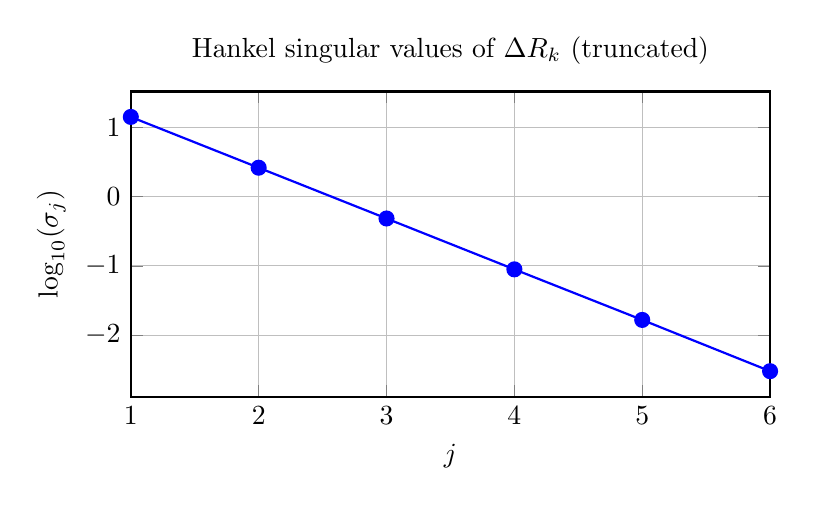
\begin{tikzpicture}
\begin{axis}[
    width=0.8\textwidth,
    height=0.45\textwidth,
    grid=both,
    thick,
    xlabel={$j$},
    ylabel={$\log_{10}(\sigma_j)$},
    title={Hankel singular values of $\Delta R_k$ (truncated)},
    xmin=1, xmax=6,
    xtick={1,2,3,4,5,6},
]
\addplot[
    color=blue,
    mark=*,
    mark size=2.5pt,
]
coordinates {
    (1, 1.15)
    (2, 0.417)
    (3, -0.316)
    (4, -1.05)
    (5, -1.78)
    (6, -2.52)
};
\end{axis}
\end{tikzpicture}
\caption{Logarithmic Hankel singular values of the residual jumps
$\Delta R_k$, using the reported values in
\eqref{eq:hankel_log_singular_values}.}
\label{fig:hankel_singular_values}
\end{figure}

\subsection{Sliding-window PCA of residuals}
\label{subsec:sliding_window_pca}

A sliding-window PCA of the residual sequence $R_k$
produces eigenvalues whose logarithms are reported as
\begin{equation}
\log_{10}(\lambda_j) \approx
0.228,\ -0.63,\ -1.49,\ -2.34,\ -3.2,\ -4.06,\ \dots
\label{eq:window_pca_log_eigenvalues}
\end{equation}
for $j=1,2,\dots$.
The variance shares are summarised as
\begin{align}
\text{PC1 variance share} &\approx 15.00\%,
\label{eq:window_PC1_share}\\
\text{PC1+PC2 variance share} &\approx 28.406\%.
\label{eq:window_PC12_share}
\end{align}

\begin{experiment}
\label{exp:window_pca}
The sliding-window PCA of $R_k$ shows that the leading principal
components explain only a modest fraction of the local variance:
about $15\%$ for PC1 and $28\%$ for PC1+PC2.
This is consistent with a relatively diffuse local geometry
for the residual sequence.
\end{experiment}

\begin{figure}[htbp]
\centering
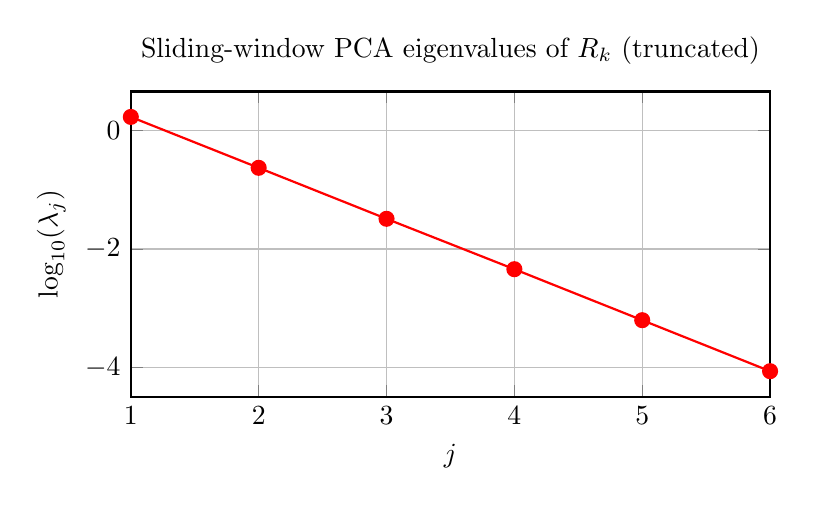
\begin{tikzpicture}
\begin{axis}[
    width=0.8\textwidth,
    height=0.45\textwidth,
    grid=both,
    thick,
    xlabel={$j$},
    ylabel={$\log_{10}(\lambda_j)$},
    title={Sliding-window PCA eigenvalues of $R_k$ (truncated)},
    xmin=1, xmax=6,
    xtick={1,2,3,4,5,6},
]
\addplot[
    color=red,
    mark=*,
    mark size=2.5pt,
]
coordinates {
    (1, 0.228)
    (2, -0.63)
    (3, -1.49)
    (4, -2.34)
    (5, -3.2)
    (6, -4.06)
};
\end{axis}
\end{tikzpicture}
\caption{Logarithmic eigenvalues from a sliding-window PCA of the residuals
$R_k$, using the reported values in
\eqref{eq:window_pca_log_eigenvalues}.}
\label{fig:window_pca_eigenvalues}
\end{figure}

\section{Summary of the raw modular excess study}
\label{sec:modular_excess_summary}

We now summarise the ``raw modular excess'' short communication,
which investigates the fractional parts $x_k$ in \eqref{eq:xk_definition}
for large samples of zeros.

\subsection{First harmonic statistic}
\label{subsec:first_harmonic_statistic}

For a sample $(x_k)$ in $[0,1)$, the study defines
\begin{align}
a &= -2 \sum_k \cos(2\pi x_k),
\label{eq:a_definition}\\
b &= 2 \sum_k \sin(2\pi x_k),
\label{eq:b_definition}\\
A &= \sqrt{a^2 + b^2},
\label{eq:A_definition}
\end{align}
and considers the fitted first harmonic
\begin{equation}
p(x) = 1 - a\cos(2\pi x) + b\sin(2\pi x),
\label{eq:p_x_definition}
\end{equation}
together with the phase of the maximum
\begin{equation}
x_{\max} = \frac{1}{2\pi} \arg(-a + i b) \pmod{1}.
\label{eq:xmax_definition}
\end{equation}

\begin{remark}
\label{rem:first_harmonic_standard}
The use of the first circular harmonic
\eqref{eq:a_definition}--\eqref{eq:xmax_definition}
is standard in the analysis of angular or modular data.
Here it is applied to the raw gap fractional parts $x_k$.
\end{remark}

\subsection{Null models}
\label{subsec:null_models}

Two scale-preserving null models are considered.
Let $h_k$ denote a local scale factor depending on $Y_{k+1}$.
The first null is a local GUE-based model,
denoted
\begin{equation}
\Delta Y_k^{\mathrm{GUE}} = h_k^{\mathrm{GUE}},
\label{eq:gue_null_definition}
\end{equation}
while the second null is a shuffled-real model that preserves
the empirical unfolded spacing distribution but destroys temporal order:
\begin{equation}
\Delta Y_k^{\mathrm{shuf}} = h_k^{\mathrm{shuf}}.
\label{eq:shuf_null_definition}
\end{equation}

\begin{remark}
\label{rem:null_model_interpretation}
The GUE-scale null \eqref{eq:gue_null_definition}
tests the agreement of the raw modular distribution with
a local random-matrix prediction.
The shuffled-real null \eqref{eq:shuf_null_definition}
is stricter: it keeps the empirical unfolded spacing distribution
and tests whether any remaining modular excess requires
temporal coupling to the slowly varying scale $h_k$.
\end{remark}

\subsection{Numerical results for the first harmonic}
\label{subsec:numerical_first_harmonic}

For $N=1{,}000{,}000$ and $N=2{,}000{,}000$ zeros,
the study reports the first-harmonic coefficient $a$
for the real gaps, the GUE-scale null, and the shuffled-real null.
The results are summarised in Table~\ref{tab:first_harmonic}.

\begin{table}[htbp]
\centering
\caption{First harmonic of raw gap fractional parts.
Z-scores compare the real value against $50$ null draws.}
\label{tab:first_harmonic}
\begin{tabular}{@{}rrrrrrr@{}}
\toprule
$N$ & $a_{\mathrm{real}}$ & $a_{\mathrm{GUE}}$ & $a_{\mathrm{shuf}}$
& $Z_{\mathrm{GUE}}$ & $Z_{\mathrm{shuf}}$ & $x_{\max}$ \\
\midrule
$1{,}000{,}000$ & $0.616383$ & $0.573036$ & $0.618266$
& $30.25$ & $-3.70$ & $0.544853$ \\
$2{,}000{,}000$ & $0.710876$ & $0.664228$ & $0.712014$
& $49.22$ & $-3.79$ & $0.519464$ \\
\bottomrule
\end{tabular}
\end{table}

For $N=2{,}000{,}000$ the relative excess over the GUE-scale null is
\begin{equation}
\frac{a_{\mathrm{real}} - a_{\mathrm{GUE}}}{a_{\mathrm{GUE}}}
\approx 7.02\%.
\label{eq:relative_excess_gue}
\end{equation}
The shuffled-real null gives
\begin{equation}
\frac{a_{\mathrm{real}} - a_{\mathrm{shuf}}}{a_{\mathrm{shuf}}}
\approx -0.16\%.
\label{eq:relative_excess_shuf}
\end{equation}

\begin{experiment}
\label{exp:first_harmonic_excess}
At $N=2{,}000{,}000$ zeros,
the real raw gaps exhibit a first-harmonic amplitude $a_{\mathrm{real}}$
about $7.02\%$ larger than the GUE-scale null $a_{\mathrm{GUE}}$,
as in \eqref{eq:relative_excess_gue}.
However, once the empirical unfolded spacings are shuffled and
remultiplied by the same local scale $h_k$,
the shuffled-real null $a_{\mathrm{shuf}}$ nearly matches
$a_{\mathrm{real}}$, with a residual difference of about $-0.16\%$
as in \eqref{eq:relative_excess_shuf}.
\end{experiment}

We include a PGFPlots figure comparing the three $a$-values
for $N=2{,}000{,}000$.

\begin{figure}[htbp]
\centering
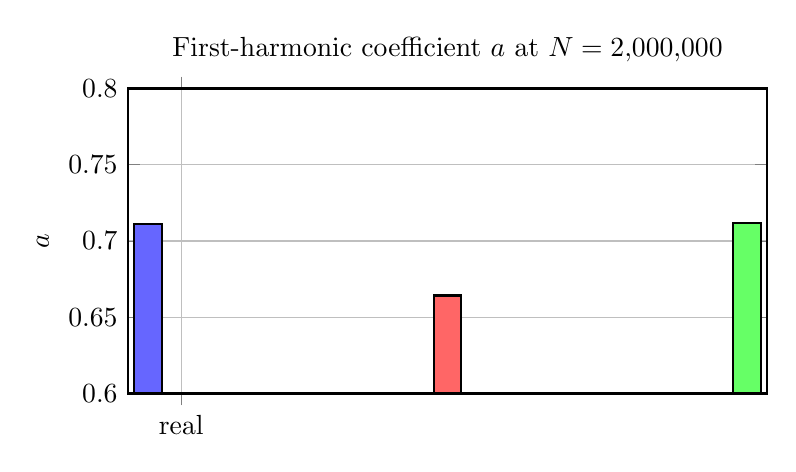
\begin{tikzpicture}
\begin{axis}[
    ybar,
    width=0.8\textwidth,
    height=0.45\textwidth,
    grid=both,
    thick,
    symbolic x coords={real,GUE,shuffle},
    xtick=data,
    ylabel={$a$},
    title={First-harmonic coefficient $a$ at $N=2{,}000{,}000$},
    ymin=0.6, ymax=0.8,
]
\addplot[fill=blue!60] coordinates {
    (real,0.710876)
};
\addplot[fill=red!60] coordinates {
    (GUE,0.664228)
};
\addplot[fill=green!60] coordinates {
    (shuffle,0.712014)
};
\end{axis}
\end{tikzpicture}
\caption{First-harmonic coefficient $a$ for the real gaps,
the GUE-scale null, and the shuffled-real null at $N=2{,}000{,}000$,
using the values in Table~\ref{tab:first_harmonic}.}
\label{fig:first_harmonic_bar}
\end{figure}

\subsection{Location of the modular peak}
\label{subsec:modular_peak_location}

The study reports that the raw gap fractional parts are more
concentrated near
\begin{equation}
x \approx 0.51946
\label{eq:modular_peak_location}
\end{equation}
than predicted by the local GUE scaling.
The absolute ordinates themselves pass a sanity check:
for $N=2{,}000{,}000$ the first harmonic amplitude of
$\log Y_k \bmod 1$ is only about $1.535\times 10^{-5}$,
indicating that the signal is located in the increments.

\begin{remark}
\label{rem:modular_peak_interpretation}
The observation \eqref{eq:modular_peak_location}
indicates a genuine modular feature of the raw gaps:
their fractional parts are not uniformly distributed modulo one
at the level of the first harmonic.
However, the shuffled-real null shows that this feature is
essentially explained by the empirical unfolded spacing distribution,
rather than by a strong temporal coupling to the local scale.
\end{remark}

\section{Integrated interpretation}
\label{sec:integrated_interpretation}

We now combine the residual/gap matrix study
(Section~\ref{sec:matrix_study_summary})
with the raw modular excess study
(Section~\ref{sec:modular_excess_summary}).

\subsection{Residual structure versus modular excess}
\label{subsec:residual_vs_modular}

The matrix study shows that:
\begin{itemize}[leftmargin=*]
\item The feature space $(dG,dRVM,dR,SG,SR)$ is effectively
two-dimensional in the PCA sense
(Experiment~\ref{exp:feature_correlation},
Remark~\ref{rem:feature_pca_rank}).
\item The Hankel singular spectrum of $\Delta R_k$
does not exhibit a dominant low-rank structure
(Experiment~\ref{exp:hankel_singular_values}).
\item The sliding-window PCA of $R_k$ has relatively diffuse
leading components
(Experiment~\ref{exp:window_pca}).
\end{itemize}
In particular, there is no evidence of a simple low-rank temporal
dynamics for the residuals.

On the other hand, the modular excess study shows that:
\begin{itemize}[leftmargin=*]
\item The raw gap fractional parts exhibit a clear first-harmonic
excess over the GUE-scale null
(Experiment~\ref{exp:first_harmonic_excess}).
\item This excess is almost entirely absorbed by the shuffled-real
null, which preserves the empirical unfolded spacing distribution
but destroys temporal order
(Equations~\eqref{eq:relative_excess_gue}
and~\eqref{eq:relative_excess_shuf}).
\end{itemize}

\begin{remark}
\label{rem:integrated_message}
Taken together, the two studies indicate that the observed raw modular
excess in zeta-zero gaps is not explained by a simple low-rank or
linearly correlated structure in the residuals $R_k$ or their jumps
$\Delta R_k$.
Instead, the excess is essentially accounted for by the empirical
unfolded spacing distribution itself.
\end{remark}

\subsection{Heuristic formulation of the main conclusion}
\label{subsec:heuristic_main_conclusion}

We now state the main conclusion in heuristic form.

\begin{heuristic}
\label{heur:main_conclusion}
Let $G_k = Y_{k+1} - Y_k$ be the raw gaps and
$x_k = \{G_k\}$ their fractional parts.
Let $R_k$ be the residuals of a smooth reference model and
$\Delta R_k$ their jumps.
The numerical evidence suggests that:
\begin{enumerate}[label=\textup{(\alph*)},leftmargin=*]
\item The sequence $(R_k)$ and its jumps $(\Delta R_k)$
do not exhibit a dominant low-rank temporal structure,
as measured by Hankel singular values and sliding-window PCA.
\item The first-harmonic excess of the modular distribution of
$(x_k)$ over a local GUE-scale null is real but small
(about $7\%$ at $N=2{,}000{,}000$ zeros).
\item This excess is almost entirely reproduced by a shuffled-real
null that preserves the empirical unfolded spacing distribution
while destroying temporal order.
\end{enumerate}
Heuristically, this indicates that the raw modular excess is
traceable to the empirical unfolded spacing law and not to
a strong temporal coupling between the residuals and the local scale.
\end{heuristic}

\begin{warning}
\label{warn:nonrigorous_status}
Heuristic~\ref{heur:main_conclusion} is based on finite-range
numerical experiments and on specific choices of null models.
It should not be interpreted as a rigorous theorem about the
asymptotic behaviour of zeta-zero gaps.
\end{warning}

\section{Open questions and future directions}
\label{sec:open_questions}

We conclude with a few questions suggested by the experiments.

\begin{question}
\label{q:residual_model_refinement}
Can one construct a refined reference model for the ordinates
$\gamma_k$ whose residuals $R_k$ have provably small Hankel rank
or controlled temporal structure, and would such a model
change the modular excess picture?
\end{question}

\begin{question}
\label{q:unfolded_spacing_theory}
Is there a theoretical framework that directly links the empirical
unfolded spacing distribution of zeta zeros to the observed
first-harmonic modular excess, beyond random-matrix heuristics?
\end{question}

\begin{remark}
\label{rem:future_work}
Future work may include:
more extensive Hankel and PCA analyses at higher heights,
alternative null models for modular statistics,
and a closer comparison with rigorous results on pair correlation
and higher-order spacing statistics
(see for instance \cite{Montgomery1973,IwaniecKowalski2004}).
\end{remark}

\begin{thebibliography}{99}

\bibitem{Titchmarsh1986}
E.~C.~Titchmarsh,
\emph{The Theory of the Riemann Zeta-Function},
2nd ed., revised by D.~R.~Heath-Brown,
Oxford University Press, 1986.

\bibitem{Edwards2001}
H.~M.~Edwards,
\emph{Riemann's Zeta Function},
Dover Publications, 2001.

\bibitem{Montgomery1973}
H.~L.~Montgomery,
The pair correlation of zeros of the zeta function,
in \emph{Analytic Number Theory},
Proc.\ Sympos.\ Pure Math.\ \textbf{24} (1973), 181--193.

\bibitem{IwaniecKowalski2004}
H.~Iwaniec and E.~Kowalski,
\emph{Analytic Number Theory},
American Mathematical Society Colloquium Publications, Vol.~53,
American Mathematical Society, 2004.

\end{thebibliography}

\end{document}
